%!TEX root = ../main.tex 

\section{Comment filtrer une alimentation?}

\subsection{Pourquoi filtrer une alimentation?}

\begin{frame}{Pourquoi Filtrer?}
    \begin{columns}
        \begin{column}{0.5\textwidth}
            \begin{center}
                \textbf{Signal Integrity}
            \end{center}
        \end{column}
        \begin{column}{0.5\textwidth}
            \begin{center}
                \textbf{Electromagnetic Interference}
            \end{center}
        \end{column}
    \end{columns}
    \begin{columns}
        \begin{column}{0.5\textwidth}
            \begin{itemize}
                \item Signaux Clean
                \item Marges d'opérations respectées
            \end{itemize}

            \centering
            \begin{tabular}{c l}
                \textcolor{UDSgreenFierte}{\faUndo}   & Rélections \\
                \textcolor{UDSgreenFierte}{\faExchange*}         & Crosstalk \\
                \textcolor{UDSgreenFierte}{\faCompress}     & Ground Bounce \\
                \textcolor{UDSgreenFierte}{\faFilter}   & \textbf{Filtration de Power} \\
            \end{tabular}
        \end{column}
        \begin{column}{0.5\textwidth}
            \begin{itemize}
                \item Passer les tests EMC
                \item Ne pas influencer d'autres circuits
                \begin{itemize}
                    \item Émissions
                    \item Immunité au bruit
                \end{itemize}

                \centering
                \begin{tabular}{c l}
                    \textcolor{UDSgreenFierte}{\faPuzzlePiece}   & Layout \\
                    \textcolor{UDSgreenFierte}{\faArrowDown}         & Grounding \\
                    \textcolor{UDSgreenFierte}{\faShield*}     & Shielding \\
                    \textcolor{UDSgreenFierte}{\faFilter}   & \textbf{Filtration de Power} \\
                \end{tabular}
            \end{itemize}
        \end{column}
    \end{columns}
\end{frame}

\begin{frame}{But d'un filtre sur l'alimentation}
    \begin{itemize}
        \item \textbf{Le but d'un filtre est de fournir le chemin de plus faible impédance vers le ground aux signaux haute-fréquence}.
        \bigskip
        \item \textbf{Le but d'un filtre est de contrôler la propagation du bruit sur l'alimentation.}
    \end{itemize}
\end{frame}

\begin{frame}{Filtration de Power}
    \begin{itemize}
        \item Tout commence avec le power
        \item Le PDN devrait constituer 25\% à 50\% de la difficulté d'un projet
        \bigskip
        \item Plein de façon de filtrer
        \item Réduire le bruit sur l'alimentation
        \item Avoir une alimentation purement DC
        \bigskip
        \item<2-> Jouer avec les impédances de mon alimentation
        \begin{itemize}
            \item<2->[] \textcolor{UDSgreenFierte}{\faEquals} ~Découplage 
            \item<2->[] \textcolor{UDSgreenFierte}{\faSync} ~Rajouter des inductances
            \item<2->[] \textcolor{UDSgreenFierte}{\faPuzzlePiece} ~Faire attention à son layout 
        \end{itemize}
        \item<2-> Ajouter des composantes actives
        \begin{itemize}
            \item<2->[] \textcolor{UDSgreenFierte}{\faRulerHorizontal} ~Régulateurs Linéaires
        \end{itemize}
    \end{itemize}
\end{frame}

\begin{frame}{D'où provient le bruit}
    \Large
    \centering
    \begin{tabular}{c l}
        \textcolor{UDSgreenFierte}{\faWaveSquare}
            & IC qui toggle \\
        [0.6em]
        \textcolor{UDSgreenFierte}{\faRoute}
            & Longues lignes de transmission \\
        \hspace{18pt}\textcolor{UDSgreenFierte}{\faExchange*}
            & \hspace{18pt}Crosstalk \\
        \hspace{18pt}\textcolor{UDSgreenFierte}{\faBroadcastTower}
            & \hspace{18pt}Antennes \\
        [0.6em]
        \textcolor{UDSgreenFierte}{\faProjectDiagram} 
            & Mauvais chemins de retour \\
        \hspace{18pt}\textcolor{UDSgreenFierte}{\faExchange*}
            & \hspace{18pt}Crosstalk \\
        \hspace{18pt}\textcolor{UDSgreenFierte}{\faStumbleupon}
            & \hspace{18pt}Ground Bounce \\
        \hspace{18pt}\textcolor{UDSgreenFierte}{\faBroadcastTower}
            & \hspace{18pt}Antennes
    \end{tabular}
\end{frame}



\subsection{Démonstration}

\subsection{Filtrer l'entrée}
\begin{frame}{L'entrée d'un système d'alimentation}
    \begin{columns}
        \begin{column}{0.66\textwidth}
            \begin{itemize}
                \item[] \textcolor{UDSgreenFierte}{\faRoute} 
                    ~Long fil qui provient d'une Power Supply
                \item[] \textcolor{UDSgreenFierte}{\faSync} 
                    ~Inductance Parasite
                \bigskip
                \item[] \textcolor{UDSgreenFierte}{\faSatelliteDish}
                    ~Pick-Up du bruit extérieur 
                \item[] \textcolor{UDSgreenFierte}{\faSignature}
                    ~Signal potentiellement bruité
                \bigskip
                \item[] \textcolor{UDSgreenFierte}{\faLongArrowAltRight}
                \textbf{~Demande de courant au travers d'une bobine.}
                \item[] \textcolor{UDSgreenFierte}{\faWaveSquare}
                \textbf{~Demande de courant non-constante}
            \end{itemize}
        \end{column}
        \begin{column}{0.33\textwidth}
            \begin{figure}
                \centering
                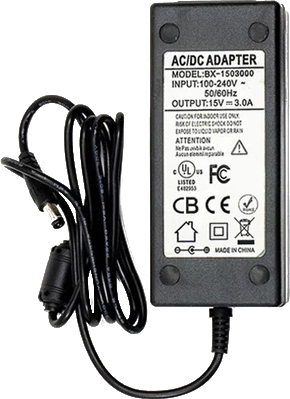
\includegraphics[width=\textwidth]{pictures/power-brick.png}
            \end{figure}
        \end{column}
    \end{columns}
\end{frame}

\begin{frame}{Découplage}
    \begin{itemize}
        \item $X_L \propto -X_C$
        \item Rajouter de la capacitance pour compenser l'inductance
        \item Plus ton fil est long, plus tu veux de capacitance
        \item Le power devrait provenir des condensateurs
        \item \textit{Couper le chemin d'inductance}
    \end{itemize}

    \pause
    \vfill
    \begin{center}
    \resizebox{0.8\textwidth}{!}{
    \ctikzset{bipoles/cuteinductor/height=0.15}
    \ctikzset{bipoles/cuteinductor/width=0.5}
    \begin{circuitikz}[american voltages]
        \draw [thick]
        (0, 0) to [short, *-] (10, 0)
        to [european resistor, l_=${LOAD}$] (10, 4)
        (0, 0) to [open, v<=$V$] (0, 4)
        to [american inductor, l=$wire$, color=red] (5, 4)
        to [short] (6, 4)
        to [cute inductor, l=$pcb$, color=UDSgreenFierte] (10, 4)
        ;

        \draw [thick] (5, 0) to [C, l=$bulk$, color=red] (5, 4);
        \draw [thick] (6, 0) to [C, l_=$decoupling$, color=UDSgreenFierte] (6, 4);

        \draw[->, thick, red]
        (1, 3.5) to [out=0, in=180] (3.5, 3.5)
        to [out=0, in=90] (4.5, 2.5);
        \draw[->, thick, UDSgreenFierte]
        (6.5, 2.5) to [out=90, in=180] (7.5, 3.5)
        to [out=0, in=180] (8.5, 3.5)
        to [out=0, in=90] (9.5, 2.5);
    \end{circuitikz}
    }
    \end{center}
\end{frame}

\begin{frame}{Filtrage avancé d'une entrée d'alimentation}
    \begin{itemize}
        \item Découplage permet de fournir un chemin de faible impédance aux signaux haute-vitesse
        \item Bulk permet d'emmagasiner des charges et que le power provienne des condensateurs et non du fil
        \bigskip
        \item<2-> \textbf{Contrôler la propagation du bruit}
        \begin{itemize}
            \item<2->[] \textcolor{UDSgreenFierte}{\faArrowRight} ~Limiter le bruit au board
            \item<2->[] \textcolor{UDSgreenFierte}{\faArrowLeft} ~Limiter le bruit hors du board
            \item<2->[] \textcolor{UDSgreenFierte}{\faFileContract} ~Passer EMC
        \end{itemize}
    \end{itemize}
\end{frame}

\begin{frame}{Rajouter des inductances}
    \begin{itemize}
        \item Rajouter de l'inductance permet de bien contrôler où va le bruit haute-fréquence.
        \item $X_L = 2\pi fL$
        \item Si $X_L > X_C$, le bruit va passer par $X_C$.
        \bigskip
        \item On vient de passer tout ce temps pour compenser l'inductance du fil d'alimentation
        \item<2-> Maintenant, on contrôle l'inductance!
        \begin{itemize}
            \item<2-> Les condensateurs de découplage fournissent la puissance haute fréquence
            \item<2-> Les condensateurs de bulk fournissent la puissance basse fréquence
            \item<2-> Les condensateurs de bulk rechargent les condensateurs de découplage
            \item<2-> L'alimentation fournit du power DC pour recharger les condensateurs de bulk
        \end{itemize}
    \end{itemize}
\end{frame}


\subsection{Filtrer la sortie d'un régulateur}
\subsection{Filtrer au IC}